\documentclass[11pt,compress,t,notes=noshow, xcolor=table]{beamer}
\input{../../style/preamble}
\input{../../latex-math/basic-math}
\input{../../latex-math/basic-ml}

\newcommand{\sens}{\mathbf{A}} % vector x (bold)

\newcommand{\batilde}{\tilde{\mathbf{a}}}
\newcommand{\Px}{\mathbb{P}_{x}} % P_x
\newcommand{\Pxj}{\mathbb{P}_{x_j}} % P_{x_j}
\newcommand{\indep}{\perp \!\!\! \perp} % independence symbol
% ml - ROC
\newcommand{\np}{n_{+}} % no. of positive instances
\newcommand{\nn}{n_{-}} % no. of negative instances
\newcommand{\rn}{\pi_{-}} % proportion negative instances
\newcommand{\rp}{\pi_{+}} % proportion negative instances
% true/false pos/neg:
\newcommand{\tp}{\# \text{TP}} % true pos
\newcommand{\fap}{\# \text{FP}} % false pos (fp taken for partial derivs)
\newcommand{\tn}{\# \text{TN}} % true neg
\newcommand{\fan}{\# \text{FN}} % false neg

\newcommand{\Tspace}{\mathcal{T}}
\newcommand{\tv}{\mathbf{t}}
\newcommand{\tj}{\mathbf{t}_j}

\usepackage{multicol}
\usepackage{color,colortbl} 
\definecolor{putblue}{RGB}{0,0,124}
\definecolor{putred}{RGB}{204,33,69}

\usetikzlibrary{mindmap,trees}
\usetikzlibrary{decorations.pathreplacing}
\usetikzlibrary{decorations.pathmorphing}
\usetikzlibrary{arrows}
\usetikzlibrary{positioning}
\usetikzlibrary{decorations.text}
\usetikzlibrary{decorations.markings}
\usetikzlibrary{decorations.shapes}
\usetikzlibrary{shapes,snakes}
\usetikzlibrary{calc,trees,positioning,arrows,chains,shapes.geometric,
	decorations.pathreplacing,decorations.pathmorphing,shapes,matrix,shapes.symbols}
\usetikzlibrary{shapes.misc}


\newcommand{\titlefigure}{figure/mean_relation}
\newcommand{\learninggoals}{
  \item Get an overview of the existing groups of methods for MTP
  \item Know that treating targets independently is often sub-optimal
%  \item 
}

\title{Advanced Machine Learning}
\date{}

\begin{document}

\lecturechapter{Methods for Multi-Target Prediction: Part 1}
\lecture{Advanced Machine Learning}



\sloppy


\begin{frame}{Independent models}
%	
	\begin{itemize}
		\item 	The most naive way to make multi-target predictions: learning a model for each target independently.
%	
	\end{itemize}

	\begin{figure}
		\centering
		\includegraphics[width=0.3\textwidth,trim = 0 0 100 100,clip]{figure/Slide13}
		\includegraphics[width=0.3\textwidth,trim = 0 0 100 100,clip]{figure/Slide14} 
%		
		$\ldots$
%		
		\includegraphics[width=0.3\textwidth,trim = 0 0 100 100,clip]{figure/Slide15}
	\end{figure}
%	
%
	\begin{itemize}
%		
		\item In multi-label classification this approach is also known as \emph{binary relevance learning.}
	%	
		\item The advantage of this approach is that it is quite easy to realize, as for single-target prediction we have a wealth of methods available.
	%
	\end{itemize}

\end{frame}

\begin{frame}{Independent Models}
%	
	\footnotesize
%	
	\begin{itemize}
%		
		\item 	We illustrate the typical approach with linear basis function model for the $m$-th target: 
		\begin{equation*}
			f(\xv)_m = \thetab_m^\intercal \phi(\xv) \,,
			\label{eq:binrel}
		\end{equation*}
%	
		where $\thetab_m$ is a target-specific parameter vector and $\phi$ some feature mapping.
        \item Remark: We do this when the number of targets is large. Otherwise, we can use normal ML modelling and model selection too.
%
		\item The parameter vectors are found by solving a (regularized) optimization problem: 
%		
		\begin{equation*}
			\label{eq:multiridge}
			\min_\Theta \|Y - \Phi \Theta \|^2_F +  \sum_{m=1}^l \lambda_m \,\|\thetab_m\|^2 \,,
		\end{equation*}
%	
		where $ \| B \|^2_F  = \sqrt{ \sum_{i=1}^n \sum_{m=1}^l B_{i,m}^2 } $ is the Frobenius norm for a matrix $B \in \R^{n \times l}$ and 
%		
		\begin{equation*}
			\label{eq:notation}
			\Phi = \begin{bmatrix} \phi(\xv^{(1)})^\top \\ \vdots \\ \phi(\xv^{(n)})^\top \end{bmatrix} \qquad \Theta = [\thetab_1 \quad \cdots \quad \thetab_l] \,.
		\end{equation*}
        Note that each column of $\Theta$ is binded with a specific target.
% 	$$Y: (n \times m) \qquad  X: (n \times p) \qquad A: (p \times m)$$
%
% 		\item The norm for regularizing the target-specific parameters can vary:
% %		
% 			\begin{itemize} \footnotesize
% %				
% 				\item L2-norm $\leadsto$ Multivariate Ridge Regression.
% %				
% 				\item L1-norm $\leadsto$ Multivariate Lasso Regression.
% %				
% %				\item Combination of 
% %				
% 			\end{itemize}
%	
	\end{itemize}
%
\end{frame}

\begin{frame}{Independent Models: Practical Performance}
%	
	The experimental results section of a typical MTP paper: 
%	
	\begin{center}
		\includegraphics[scale=0.45, trim = 0 50 0 100,clip]{figure/barplots} \\
	\end{center}
%
	$\leadsto$ Independent models do not exploit target dependencies compared to more sophisticated methods, which seems to be a key for better performance in MTP problems.
%	
\end{frame}


\section{Similarity-enforcing methods}

\begin{frame}[t]
	\frametitle{Mean-regularized multi-task learning}
	
	\vspace{0.2cm}
	\begin{columns}
		\column{5cm}
		\footnotesize{
			\begin{itemize} 
%				
				\item \emph{Idea}: The models for the different targets should behave similar. How?
%				One can enforce similarity of the parametrizations of the models for the different targets.
%				
				\item \emph{Simple solution}: The parameters of these models should have similar values.
%				
				\item \emph{Approach}: Bias the parameter vectors towards their overall mean vector:
					\vspace{0.2cm}
				\begin{equation*}
					\label{eq:meanreg}
					\min_\Theta \|Y - \Phi \Theta \|^2_F + \lambda \sum\nolimits_{m=1}^l \|\thetab_m - \frac{1}{l} \sum\nolimits_{m'=1}^l \thetab_{m'} \|^2 \, ,
				\end{equation*}
%				
				\item \emph{Disadvantage}: The assumption of all target models being similar might be invalid for many applications. \lz
			\end{itemize}
		}
		\column{4.5cm}
		
		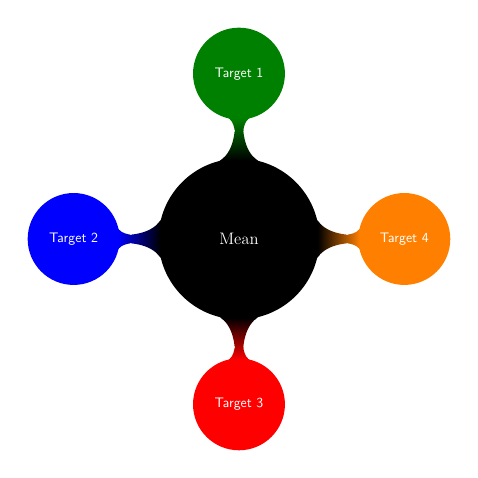
\begin{tikzpicture}[
			level 1 concept/.append style={font=\sf, level distance = 21mm},
			level 2 concept/.append style={font=\sf, level distance = 21mm},
			every node/.append style={scale=0.5}]
			
			\path[mindmap, concept color=black,text=white]
			
			node[concept] {Mean}
			child[grow = 90, concept color=green!50!black] { node[concept] {Target 1}}
			child[grow = 180,concept color=blue] { node[concept] {Target 2}}
			child[grow = 270,concept color=red] { node[concept] {Target 3} }
			child[grow = 360,concept color=orange] { node[concept] {Target 4} };   
		\end{tikzpicture}
%	
	\end{columns}

{\tiny Evgeniou and Pontil, Regularized multi--task learning, KDD 2004}
\end{frame}


%\begin{frame}{Joint feature selection}
%	\small
%\begin{itemize}
%%	
%\item Enforce that the same features are selected for different targets:
%$$
%\min_A \|Y - XA \|^2_F +  \sum_{i=1}^p \lambda_j \|\ba^{(i)} \|^2  
%$$   
%%
%\item The vectors $\ba^{(i)}$ now represent the columns of matrix $A^T$:
%%
%\end{itemize}
%\begin{center}
%\includegraphics[width=0.9\textwidth,trim = 0 240 30 50,clip]{figure/Dia21}
%\end{center}
%%
%\begin{itemize}
%	%	
%	\item Using L1-norm or a combination of L1- and L2-norm can lead to sparsity.
%%	
%\end{itemize}
%%
%	{\tiny Obozinski et al., Joint covariate selection and joint subspace selection for multiple classification problems. Statistics and Computing 2010.}
%\end{frame}


\begin{frame}
	\frametitle{Stacking (Stacked generalization)}
	
	\begin{itemize}
%		
		\item Originally introduced as a general ensemble learning or blending technique.
%		
		\item Level 1 learners: apply a series of ML methods on the same dataset (or, one ML method on bootstrap samples of the dataset)
		\item Level 2 learner: apply an ML method to a new dataset consisting of the predictions obtaining at Level 1 
	\end{itemize}
	
	\begin{center}
		\def\layersep{1.25cm}
		\begin{tikzpicture}[shorten >=1pt,->,draw=black!50, node distance=\layersep]
			\tikzstyle{every pin edge}=[<-,shorten <=1pt]
			\tikzstyle{neuron}=[circle,fill=black!25,minimum size=17pt,inner sep=0pt]
			\tikzstyle{input neuron}=[neuron, fill=green!50];
			\tikzstyle{output neuron}=[neuron, fill=red!50];
			\tikzstyle{hidden neuron}=[neuron, fill=blue!50];
			\tikzstyle{annot} = [text width=4em, text centered]
			
			% Draw the input layer nodes
			\foreach \name / \y in {1,...,4}
			% This is the same as writing \foreach \name / \y in {1/1,2/2,3/3,4/4}
			\node[input neuron] (I-\name) at (\y, 0) {$f_\y$};
			
			% Draw the hidden layer nodes
			\foreach \name / \y in {1}
			% \path%[yshift=0.5cm]
			\node[hidden neuron] (H-\name) at (2.5, \layersep) {$h_\y$};
			
			
			% % Draw the output layer node
			\node[output neuron] (I) at (2.5, -\layersep) {$\xv$};
			%%
			%%    % Connect every node in the input layer with every node in the
			%%    % hidden layer.
			\foreach \source in {1,...,4}
			\foreach \dest in {1}
			\path (I-\source) edge (H-\dest);
			%%
			%    % Connect every node in the hidden layer with the output layer
			\foreach \source in {1,...,4}
			\path (I) edge (I-\source);
			%
			% Annotate the layers
			\node[annot,left of=H-1, node distance=3cm] (hl) {Level 2}; 
			\node[annot,below of=hl, node distance=\layersep] {Level 1};
			%%    \node[annot,right of=hl] {Output layer};
		\end{tikzpicture}
	\end{center}
	{\tiny Wolpert, Stacked generalization. Neural Networks 1992.}
	%D. Wolpert, Stacked Generalization, Machine Learning, 1992
\end{frame}

\begin{frame}
	\frametitle{Stacking applied to MTP }
	\footnotesize
	\begin{columns}
		\begin{column}{4.5cm}
			\begin{itemize}
%				
				\item Level 1: learn a model for every target independently
                \vspace{5pt}
%				
				\item   [$\leadsto$] $f(\xv)_1,\ldots,f(\xv)_l$
%				
				\item Level 2: learn a model for every target independently, using the predictions of the first step
%				
				\item   [$\leadsto$] $f(\xv) = g(f(\xv)_1,\ldots,f(\xv)_l)$ \\
				Or: $f(\xv) = g(f(\xv)_1,\ldots,f(\xv)_l,\xv)$  \\
%				
%				 
			\end{itemize}
		\end{column}
		
		\begin{column}{5cm}
			\def\layersep{2cm}
			\begin{tikzpicture}[shorten >=1pt,->,draw=black!50, node distance=\layersep]
				\tikzstyle{every pin edge}=[<-,shorten <=1pt]
				\tikzstyle{neuron}=[circle,fill=black!25,minimum size=17pt,inner sep=0pt]
				\tikzstyle{input neuron}=[neuron, fill=green!50];
				\tikzstyle{output neuron}=[neuron, fill=red!50];
				\tikzstyle{hidden neuron}=[neuron, fill=blue!50];
				\tikzstyle{annot} = [text width=4em, text centered]
				
				% Draw the input layer nodes
				\foreach \name / \y in {1,...,4}
				% This is the same as writing \foreach \name / \y in {1/1,2/2,3/3,4/4}
				\node[input neuron] (I-\name) at (\y, 0) {$f_\y$};
				
				% Draw the hidden layer nodes
				\foreach \name / \y in {1,...,4}
				% \path%[yshift=0.5cm]
				\node[hidden neuron] (H-\name) at (\y, \layersep) {$g_\y$};
				
				
				% % Draw the output layer node
				\node[output neuron] (I) at (2.5, -\layersep) {$\xv$};
				%%
				%%    % Connect every node in the input layer with every node in the
				%%    % hidden layer.
				\foreach \source in {1,...,4}
				\foreach \dest in {1,...,4}
				\path (I-\source) edge (H-\dest);
				%%
				%    % Connect every node in the hidden layer with the output layer
				\foreach \source in {1,...,4}
				\path (I) edge (I-\source);
				%
				% Annotate the layers
				\node[annot,left of=H-1, node distance=1cm] (hl) {Level 2}; 
				\node[annot,left of=I-1, node distance=1cm] {Level 1};
				%%    \node[annot,right of=hl] {Output layer};
			\end{tikzpicture}
		\end{column}
	\end{columns}
%
	\begin{itemize}
%		\item 
		\item Advantages: Easy to implement and general. 
        \vspace{5pt}
        
		\item Has been shown to avoid overfitting in multivariate regression.
        \vspace{5pt}
        
		\item If level 2 learner uses regularization $\leadsto$ models are forced to learn similar parameters for different targets.  
	\end{itemize}
	% 
	{\tiny Cheng and H\"ullermeier, Combining Instance-based learning and Logistic Regression for Multi-Label classification, Machine Learning, 2009.}
	
\end{frame}

\begin{frame}{Enforcing similarity in (Deep) Neural Networks}
	\small
	\begin{center}
		Commonly-used architecture: weight sharing in the final layer with $m$ nodes, i.e., weight sharing among the targets \\
		\vspace{0.2cm}
		\includegraphics[scale=0.4]{figure/weightsharing}
	\end{center}

{\tiny Caruana, Multitask learning: A knowledge-based source of inductive bias. Machine	Learning 1997.}
\end{frame}


%
\endlecture
\end{document}
